\documentclass[a4paper,12pt]{article}
\usepackage[utf8]{inputenc}
\usepackage{listings}
\usepackage[margin=1in]{geometry}
\setlength\parindent{0pt}
\usepackage{xcolor}
\usepackage{graphicx}
\definecolor{dkgreen}{rgb}{0,0.6,0}
\definecolor{dred}{rgb}{0.545,0,0}
\definecolor{dblue}{rgb}{0,0,0.545}
\definecolor{lgrey}{rgb}{0.9,0.9,0.9}
\definecolor{gray}{rgb}{0.4,0.4,0.4}
\definecolor{darkblue}{rgb}{0.0,0.0,0.6}
\lstdefinelanguage{cpp}{
      backgroundcolor=\color{lgrey},  
      basicstyle=\footnotesize \ttfamily \color{black} \bfseries,   
      breakatwhitespace=false,       
      breaklines=true,               
      captionpos=b,                   
      commentstyle=\color{dkgreen},   
      deletekeywords={...},          
      escapeinside={\%*}{*)},                  
      frame=single,                  
      language=C++,                
      keywordstyle=\color{purple},  
      morekeywords={BRIEFDescriptorConfig,string,TiXmlNode,DetectorDescriptorConfigContainer,istringstream,cerr,exit}, 
      identifierstyle=\color{black},
      stringstyle=\color{blue},      
      numbers=right,                 
      numbersep=5pt,                  
      numberstyle=\tiny\color{black}, 
      rulecolor=\color{black},        
      showspaces=false,               
      showstringspaces=false,        
      showtabs=false,                
      stepnumber=1,                   
      tabsize=5,                     
      title=\lstname,                 
    }
    
%opening
\title{CS165 Assignment 7}
\author{Jason Dorweiler}

\begin{document}

\maketitle

\section{Requirements and Possible Solution}

For part one of the assignment I will have to create a program that will plot the number outcomes of several random dice rolls.  The plot will be in the form of a histogram.  To solve this problem I will have to use some of the complex data types from STL and Boost, such as, maps, vectors, and lists.  \\

I think the possible solution for the first part shouldn't be too hard.  The videos this week go over pretty much this exact same problem.  A rough example for how I think this will work:

  \begin{lstlisting}[language=cpp,caption={code for pt 1}]
  //we need random numbers so seed the PRNG
  boost::mt19937 gen(std::time(NULL));
  
  //assuming we have input for the number number of dice and rolls.
  //we will roll all the dice at once and keep track of the  total. 
  //store in a map
  
  for(i=0;i<number of rolls){ //for each roll
  	for(j-0;j<number of dice){ //for each die
  		total += rng(); //total for each roll
  	}
  }
  
  //then using the total check to see if it is in the map
  //if it isn't then add it, if it is then increment.
  
  if(map.find(total) == map.end()){
  	map.[total] = 0; //not in the map yet set to 0
  }
  ++map[value]; //add one
  
  \end{lstlisting}
  
That will give a map that will contain the totals of each roll and the number of times it was seen which I can plot out as a histogram. 

For part two I will have to take the code posted on blackboard and modify it to accept an arbitrary number of dice and sides on the dice. The added extra practice part also asks to allow for each specific die to have a different number of sides.  \\

I'll go for the implementation where each die has a different number of sides.  This seems like a perfect time to use a dice class.  That way I can have each single die created with a private number of sides.  An example of how that might look:

  \begin{lstlisting}[language=cpp,caption={Dice class}]
  class dice{
  	public:
  		constructors & destructor here
  		
  		int GET_Sides(){
  			return this->number_of_sides
  		}
  		
  	private:
  		int number_of_sides
  }
   
  \end{lstlisting}

Then using code similar to the first part I can ask for the number of sides on each specific die and use that for figuring out the total of each roll. 

\section {Implementation}

My implementation for part one of this assignment stuck pretty much to what I had planned.  I was a bit confused on part two because I was looking at the wrong source file.  I didn't notice the update on blackboard about the wrong file being shown until after I finished.  Anyway I ended up just writing a single program that asks for the number of dice, the number of sides for each, and then the number of rolls.  This seems at least to me to cover the requirement for both part one and part two of the assignment. \\

I ended up using the dice class to represent a die with an specific number of sides.  This class sets the number of sides to zero with a default constructor.  Then a member function called $rollDie()$ is used to generate a random number in the range of $1\rightarrow NumberOfSides$. 

  \begin{lstlisting}[language=cpp,caption={Returning a random int from the dice class}]
          int rollDie(){ //Roll the die and return a random in
          				//based on the number of sides.
            int value;
            // set the uniform distribution from 1 to the number of sides
            // generate a random number in that range and return it.
            boost::uniform_int<> dist(1,sides);
            boost::variate_generator<boost::mt19937&,
                boost::uniform_int<> > rng(gen, dist);

            value = rng();
            return value;
        }
  \end{lstlisting}

With the dice class able to return a random number for each specific die it wasn't too hard to modify to increment the total of each roll based on this random number.\\

To plot the histogram I first just made a simple loop that printed on the bars horizontally.  That was kind of boring looking and I did end up taking a look at the hint code posted which shows how to plot a vertical histogram.

I borrowed some ideas from that and noticed the neat way of doing an IF statement inside of an output stream.  For an example I use that to for printing out the y-axis.\\

  \begin{lstlisting}[language=cpp,caption={Inline IF statements}]
	    std::cout << " " << max-i << ((max-i < 10) ? " -|":"-|");
  \end{lstlisting}
  
This line is an in-line IF statement that checks to see if the number being printed is less than 10.  If it is then it prints out the y-axis bar with an extra space to make up for  the number having less than two digits. \\

The plot histogram function works by taking the total number of rolls and normalizing to get a percentage for each total.  Then the histogram is created by pushing back each row filled with 1s. This creates a histogram of 1s that could be plotted horizontally.  Plotting the histogram vertically is then done by looping from the max percent down and checking to see if the spot in the histogram is true or false.  If it is true then plot a coloured block.  It it is false then just plot an empty space. \\

The colors are generated using ANSI escape characters.  I stored these in a separate vector mostly just to keep them modular. These could also have been generated inside of the histogram plotting function. \\

  \begin{lstlisting}[language=cpp,caption={Generating color ansi excape strings}]
void makeColors(std::map<int, std::string> &colors, int totalSides){
    for(int i = 0; i < totalSides; ++i){
        int colorCode = i%6+1;
        // static cast to long long so it works on flip.. 
        colors[i] = "\033[0;4"+std::to_string(static_cast<long long>(colorCode))+"m";

    }
}

  \end{lstlisting}
  
It works by generating an escape string based on the starting string for coloured ANSI and incrementing through the 6 colors in the loop by using $i \% 6+1$.  This skip printing in black.  It also uses the $std::to\_string$ function which I learned I had to cast as a long long to get it to work on flip.  I included a picture of the output below just in case it doesn't print correctly on some other compiler. 

\begin{figure}[h!]
\centering
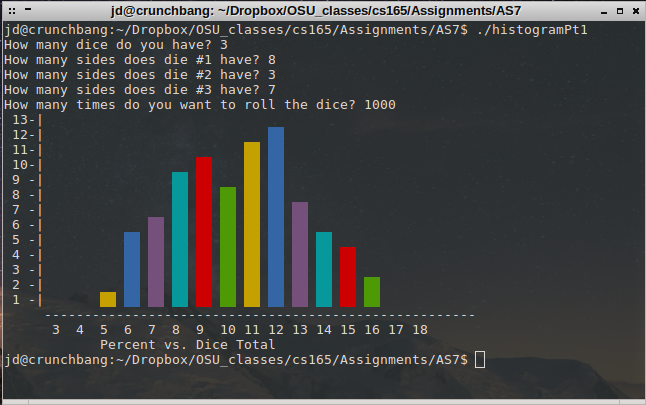
\includegraphics[width=0.8\textwidth]{hist}
\caption{Awesome Image}
\end{figure} 

\newpage

I made changes to the histogram.cpp file for part 2 of the assignment.  These were mostly just copy pasta changes using the code I made for part 1 which was already explained. 


\section{Reflection}

This assignment wasn't too tricky.  The more complex data containers seem at least to me to be way easier to use.  I like arrays and all but I'll stick to vectors unless I really really need an array. 

I do like the more open-ended nature of this assignment.  Making a nice plot like this was actually a problem I had been thinking about since the integral calculation assignment.  I had been trying to think of way to make a visual plot of the Riemann sum integral.  Doing this at the time was a bit over my head but not any more!  Maybe that's a good add on for the next group of students?\\



\end{document}
